%
% beugung-herleitung.tex -- Herleitung aus WsComm2-Vorlesung
%
%
% !TEX root = ../../buch.tex
% !TEX encoding = UTF-8
%

\noindent
Die Fresnel-Integrale sind häufig in der Wellentheorie und in der Analysis anzutreffen. 
Sie sind nützlich, um die Ausbreitung von Wellen durch Beugung zu berechnen. 
In der drahtlosen Kommunikation können mithilfe der Fresnel-Integrale die Feldstärke 
\index{drahtlose Kommunikation}%
\index{Feldstarke@Feldstärke}%
und damit die Intensität elektromagnetischer Wellen hinter einem Hindernis 
\index{elektromagnetische Wellen}%
unter Berücksichtigung der Beugung berechnet werden. 
\index{Beugung}%
Die komplexe Analysis hilft dabei, die Intergrale in ein einfacheres Integral zusammenzufassen. 

\section{Definition}
\kopfrechts{Definition}

Die eigentlichen Fresnel-Integrale sind definiert als 
\index{Fresnel-Integral!eigentlich}%
\begin{equation}
    C(v) 
    = 
    \int_{0}^{v} \cos \biggl(\frac{\pi}{2}t^2\biggr) \,dt
    \qquad \text{und} \qquad
    S(v) 
    = 
    \int_{0}^{v} \sin \biggl(\frac{\pi}{2}t^2\biggr) \,dt.
    \label{fresnel:integral-C-S}
\end{equation}
Direkt geplottet verhalten sie sich wie in Abbildung~\ref{fresnel:C-S-Plot}
dargestellt.
%
% fig-cs.tex
%
% (c) 2026 Prof Dr Andreas Müller
%
\begin{figure}
\centering
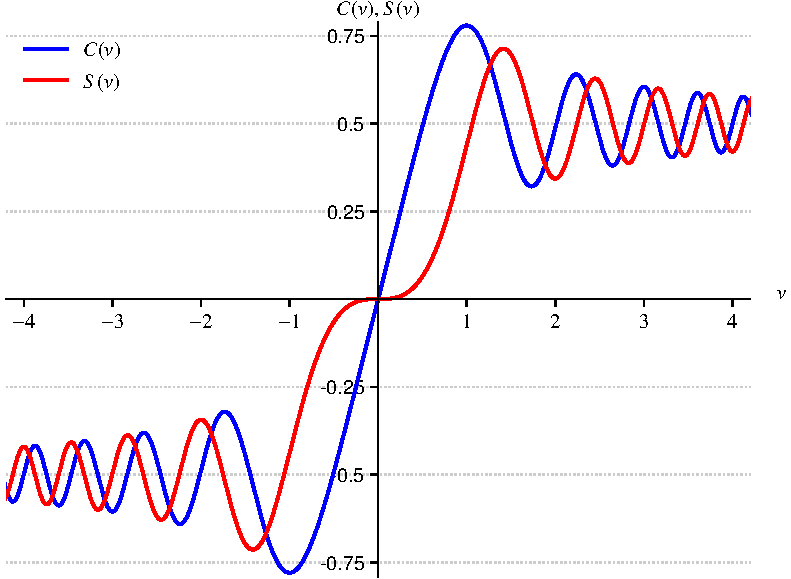
\includegraphics[width=\textwidth]{papers/fresnel/pgf/fresnel-c-s.pdf}
\caption{$C$-$S$-Plot
\label{fresnel:C-S-Plot}}
\end{figure}

Für $v\to\infty$ bleiben beide Integrale beschränkt und scheinen gegen den endlichen Wert
\begin{equation}
    \lim\limits_{v \to \infty} C(v)
    =
    \lim\limits_{v \to \infty} S(v)
    =
    \frac{1}{2} 
\end{equation}
zu konvergieren.
Der Grenzwert für $v\to\infty$ wird als uneigentliches Fresnel-Integral
bezeichnet.
\index{Fresnel-Integral!uneigentlich}%
Beide Integrale können auch gemeinsam als komplexe Funktion 
\begin{equation}
    F(v)=C(v) + jS(v)
    \label{fresnel: Komplexe Funktion}
\end{equation}
geschrieben werden.
Die daraus resultierende Kurve in der komplexen Ebene ist eine Spirale,
die in Abbildung~\ref{fresnel:Cornu-Spirale} dargestellt ist. Sie heisst
auch die \emph{Cornu-Spirale}.
\index{Cornu-Spirale}%

%
% fig-cskomplex.tex
%
% (c) 2026 Prof Dr Andreas Müller
%
\begin{figure}
\centering
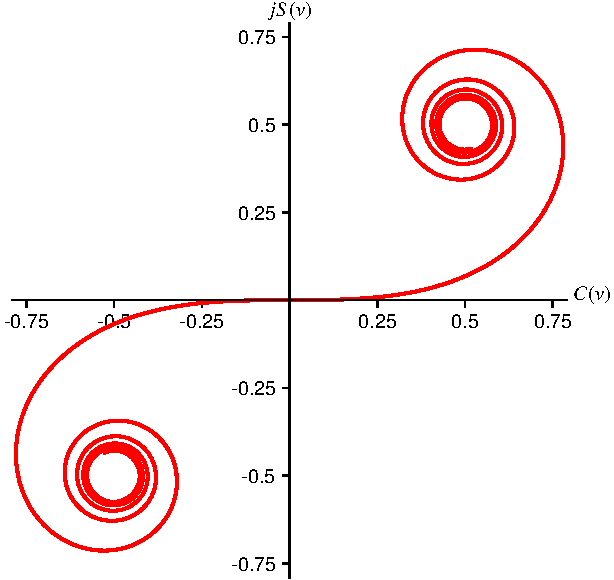
\includegraphics{papers/fresnel/pgf/fresnel-c-s-komplex.pdf}
\caption{Cornu-Spirale in der komplexen Ebene.
\label{fresnel:Cornu-Spirale}}
\end{figure}


\section{Komplexe Analysis zur Integrallösung}
\kopfrechts{Komplexe Analysis zur Integrallösung}
Als nächstes wird das uneigentliche Integral der Fresnel-Integrale gelöst.
\index{Fresnel-Integral}%
Nach der Euler-Formel
\index{Euler-Formel}%
\[
e^{j\vartheta}
=
\cos \vartheta + j \sin \vartheta
\]
kann die in \eqref{fresnel: Komplexe Funktion} definierte Funktion $F(v)$ in die komplexe Form
\begin{equation}
    F(v \to \infty)
    =
    \int_{0}^{v} e^{j \pi t^2 / 2} \,dt
    =
    \int_{0}^{v} f(t) \,dt
    \qquad
    \text{mit}
    \;
    f(t) = e^{j\pi t^2/2}
    \label{fresnel:fresnel-komplexe-form}
\end{equation}
umgeschrieben werden, welche zugleich auch holomorph ist.
Diese Umstellung des uneigentlichen Integrals erlaubt es, den Integralsatz von Cauchy anzuwenden.
\index{Satz!Integralsatz von Cauchy}%
Statt auf der reellen Achse zu integrieren,
wo die Funktion stark oszilliert,
kann der Integrationsweg gedreht werden,
z.\,B. um $45^{\circ}$.
Daraus entsteht ein einfacher integrierbares Gauss-Integral.
\index{Gauss-Integral}%

\subsection{Drehung für Cauchy-Integral}\label{fresnel:Drehung-Cauchy}
Mit einer neuen Funktion, welche die Funktion $t$ um $\ang{45}$ dreht, erhält man 
\begin{equation}
    t 
    = 
    e^{j \pi / 4} u,
    \quad
    dt 
    = 
    e^{j \pi / 4} \,du.
    \label{fresnel:komplexe-form-substitution}
\end{equation}
Da $t$ im Integranden von \eqref{fresnel:fresnel-komplexe-form} im Quadrat vorkommt, wird die neue Funktion von
\[
t^2
=
e^{j \pi / 2} u^2
=
j u^2
\]
abhängen. 
Daraus folgt nun, 
dass der Integrand des Integrals \eqref{fresnel:fresnel-komplexe-form}
\begin{equation}
    e^{j \pi t^2 / 2}
    =
    e^{-u^2 \pi / 2}
    \label{fresnel:komplexer-term-umstellung}
\end{equation}
wird.

\subsection{Rechtfertigung für die Drehung}
Die Drehung sorgt dafür,
dass der Integrationsweg von der reellen Achse aus
um $\ang{45}$ nach oben gedreht wird,
wie in der Abbildung~\ref{fresnel:drehung-rechtfertigung} ersichtlich.
Cauchys Integralsatz besagt, dass
\begin{equation}
    \underbrace{\int_{0}^{R} f(t) \,dt}_{\text{\textcolor{green!50!black}{horizontal}}}
    =
    \underbrace{e^{j\pi/4}
    \int_{0}^{R} f(e^{j\pi/4} u) \,du}_{\text{\textcolor{orange!90!black}{gedreht}}}
    -
    \underbrace{\int_{\text{Kreisbogen}} f(R) \,dR.}_{\text{\textcolor{blue!50!black}{Bogen}}}
\end{equation}
% mit den korrespondierenden Farben in der Darstellung.
Falls also der Beitrag des Bogenintegrals für $R \to \infty$ verschwindet,
dürfen wir die Substitution aus dem Abschnitt~\ref{fresnel:Drehung-Cauchy}
verwenden. 

Für den Kreisbogen mit Radius $R$ brauchen wir eine Funktion,
welche als
\begin{equation}
    t
    =
    R\cdot e^{j\vartheta},
    \qquad
    t^2
    =
    R^2\cdot e^{2j\vartheta},
    \qquad
    0 \leq \vartheta \leq \frac{\pi}{4}.
\end{equation}
definiert ist.
Um den Kreisbogen mit dem Integrand aus der 
Gleichung~\eqref{fresnel:fresnel-komplexe-form} vergleichen zu können,
setzen wir den Faktor $\frac{j\pi}{2}$ auf beiden Seiten ein wie
\begin{subequations}
    \begin{align}
        \frac{j\pi t^2}{2}
        &=
        \frac{j\pi R^2}{2}
        \underbrace{\left(\cos(2\vartheta) + j \sin(2\vartheta)\right)}_{\displaystyle e^{2j\vartheta}}\\
        &=
        -\frac{\pi R^2}{2}\sin(2\vartheta) + j\frac{\pi R^2}{2}\cos(2\vartheta).
    \end{align}
\end{subequations}
Für den Betrag der Bogenfunktion erhalten wir
\begin{equation}
    |f(R)|
    =
    \exp\biggl(-\frac{\pi R^2}{2}\sin(2\vartheta)\biggr).
\end{equation}
Für unsere Anwendung geht $R \to \infty$.
Der Betrag der Bogenfunktion fällt exponentiell ab, 
während die Länge des Bogens linear wächst.
Der Bogen selbst verschwindet zwar nicht,
aber sein Einfluss auf den gesamten Integralbetrag,
an dem wir interessiert sind, schon.
Dementsprechend dürfen wir die Substitution anwenden.

%
% fig-drehung.tex
%
% (c) 2026 Prof Dr Andreas Müller
%
\begin{figure}
\centering
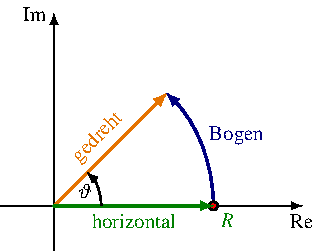
\includegraphics{papers/fresnel/images/drehung.pdf}
\caption{Integrationswege in der komplexen Ebene mit Radius $R$.
\label{fresnel:drehung-rechtfertigung}}
\end{figure}


\subsection{Integrierung der Drehung}
Aus den Gleichungen \eqref{fresnel:komplexe-form-substitution} 
und \eqref{fresnel:komplexer-term-umstellung} erhält man das substituierte Integral
\[
F(u \to \infty)
=
e^{j \pi / 4}
\int_{0}^{\infty} e^{-\pi u^2 / 2} \,du.
\]
Das Integral ist das bekannte Gauss-Integral
\begin{equation}
    \int_{0}^{\infty} e^{-au^2} \,du 
    =
    \frac{1}{2}
    \sqrt{\dfrac{\pi}{a}},
    \quad
    a > 0.
    \label{fresnel:gauss-integral}
\end{equation}
Mit dem Vorfaktor $a=\frac{\pi}{2}$ erhält man dementsprechend
\[
F(u \to \infty)
=
e^{j \pi / 4}
\frac{1}{2}
\sqrt{\dfrac{\pi}{\pi / 2}}
=
e^{j \pi / 4}\frac{1}{\sqrt{2}}.
\]
Der Exponentialfaktor vor dem Bruch ist 
\[
e^{j \pi / 4}
=
\dfrac{1 + j}{\sqrt{2}},
\]
womit sich das Integral zu
\begin{equation}
    F(u \to \infty)
    =
    \frac{1 + j}{2}
    =
    \frac{1}{2} + j\frac{1}{2}
    \label{fresnel:integral-subst-gelöst}
\end{equation}
vereinfacht.

\subsection{Übergang zur Fresnel-Funktion}
Schreibt man das Integral \eqref{fresnel:integral-subst-gelöst} wieder mit der Euler-Formel um,
können der Realteil
\[
\int_{0}^{\infty} \cos \biggl(\frac{\pi}{2}t^2\biggr)\, dt
=
\frac{1}{2}
\]
und der Imaginärteil
\[
\int_{0}^{\infty} \sin \biggl(\frac{\pi}{2}t^2\biggr)\, dt
=
\frac{1}{2}
\]
abgelesen werden.
Dadurch ergibt sich
\[
C(v \to \infty) = S(v \to \infty) = \dfrac{1}{2},
\]
was am Anfang graphisch schon angedeutet wurde.
